%=====================================================================%
% DOCUMENT DEFINITION
%=====================================================================%


\documentclass[12pt]{article}

\usepackage[magyar]{babel}
\usepackage[T1]{fontenc}

\usepackage{subcaption}

\usepackage{gensymb}

\usepackage{setspace}
\onehalfspacing

\usepackage[
    a4paper,
    top=2cm,
    bottom=2cm,
    left=2cm,
    right=2cm,
    marginparwidth=1.75cm
]{geometry}

\usepackage[skip=8pt plus1pt, indent=20pt]{parskip}

% inserting images
\usepackage{graphicx}
\usepackage{float}
\graphicspath{{images/}}

% references
%\usepackage{csquotes}
%\usepackage[
%    backend=biber,
%    style=numeric-comp,
%    sorting=none
%]{biblatex}
%\addbibresource{references.bib}


% math
\usepackage{amsmath}
\usepackage{empheq}

% tables
\usepackage{booktabs}

% color
\usepackage{xcolor}

% dummy text
\usepackage{lipsum}

%=====================================================================%
% DOCUMENT
%=====================================================================%
\setlength{\parindent}{0pt} 


\begin{document}

%=====================================================================%
% TITLE PAGE
%=====================================================================%

\begin{titlepage}

\centering
\singlespacing

% ------------------------------------------------
% UNIVERSITY LOGO
% ------------------------------------------------

\includegraphics[width=0.70\textwidth]{bmelogo.png}

\vspace{0.4cm}

{\Large\bfseries
Budapesti Műszaki és Gazdaságtudományi Egyetem\par}

\vspace{0.15cm}

{\Large Gépészmérnöki Kar\par}

% ------------------------------------------------
% TITLE
% ------------------------------------------------

\vspace{2cm}

{\LARGE\bfseries
Megújuló energiaforrások technológiái: \\
Geotermikus erőmű villamosenergia-termelésre\par}

\vspace{0.3cm}

{\Large Projekt Dokumentáció\par}

% ------------------------------------------------
% DATE
% ------------------------------------------------

\vspace{1cm}

{\Large 2026/27/1\par}

% ------------------------------------------------
% LAB RESPONSIBLE
% ------------------------------------------------

\vspace{1cm}

{\Large
\underline{Tárgyfelelős}\\[-0.05cm]
\textbf{Dr. Mayer Martin János}
\par}

% ------------------------------------------------
% STUDENTS
% ------------------------------------------------

\vfill

\begin{minipage}[t]{0.47\textwidth}
    \centering

    {\Large {Hallgató}\par}

    \vspace{0.1cm}

    {\bfseries
    név (neptun kód)\par}
     {\normalsize
    szak\par}
    {\normalsize
    email}
    
\end{minipage}
\hfill
\begin{minipage}[t]{0.47\textwidth}
    \centering

    {\Large {Hallgató}\par}
   

    \vspace{0.1cm}

    {\bfseries
    név (neptun kód)\par}
     {\normalsize
    szak\par}
    {\normalsize
    email}
    
    
\end{minipage}

\vspace{0.5cm}

\begin{minipage}[t]{0.47\textwidth}
    \centering

    {\Large {Hallgató}\par}

    \vspace{0.1cm}

    {\bfseries
    név (neptun kód)\par}
     {\normalsize
    szak\par}
    {\normalsize
    email}
    
\end{minipage}
\hfill
\begin{minipage}[t]{0.47\textwidth}
    \centering

    {\Large {Hallgató}\par}
   

    \vspace{0.1cm}

    {\bfseries
    Hanna ERTL (SPH4U7)\par}
    {\normalsize
    Fizikus-mérnök BSc\par}
    {\normalsize
    hannavedaertl@gmail.com}
    
    
\end{minipage}

\vspace{1cm}

\end{titlepage}


%=====================================================================%
% REPORT STARTS HERE
%=====================================================================%

\newpage \section{Szeged Térségi Geotermikus Erőmű} 

\newpage \section{ORC Termodinamikai Modell}

\newpage \section{Éves Dinamikus Szimuláció és Optimalizálás}
Az ORC termodinamikai modellre építve elvégeztük a rendszer 8760 
órás éves dinamikus szimulációját a három kiválasztott munkaközeg 
(R245fa, R1233zd(E), R600a) elpárolgási nyomásának optimalizálására. 
Az 1. táblázat összefoglalja az optimális nyomásértékeket, valamint a 
megtermelt villamos energia éves összegét, átlagát és szélsőértékeit. 
A napi ingadozások kisimítására és az éves trendek szemléltetésére 168 
órás gördülő átlagot alkalmaztunk.

\begin{table}[htbp]
    \centering
    \label{tab:orc_annual_summary}
    \vspace{2mm}
    \renewcommand{\arraystretch}{1.3}
    \resizebox{\textwidth}{!}{%
    \begin{tabular}{|l|c|c|c|c|c|}
        \hline
        \textbf{Munkaközeg} & 
        \shortstack{\textbf{Optimális} $\boldsymbol{p_{\text{evap}}}$ \\ $[\text{bar}]$} & 
        \shortstack{\textbf{Éves termelés} \\ $[\text{MWh}]$} & 
        \shortstack{\textbf{Átlagos} $\boldsymbol{P_{\text{nettó}}}$ \\ $[\text{MW}]$} & 
        \shortstack{\textbf{Csúcs} $\boldsymbol{P}$ \textbf{(tél)} \\ $[\text{MW}]$} & 
        \shortstack{\textbf{Min} $\boldsymbol{P}$ \textbf{(nyár)} \\ $[\text{MW}]$} \\
        \hline
        R245fa     & 6.69  & 53\,793.48 & 6.14 & 9.45 & 1.21 \\ \hline
        R1233zd(E) & 5.59  & 52\,987.82 & 6.05 & 9.27 & 1.21 \\ \hline
        R600a      & 12.02 & 53\,733.66 & 6.13 & 9.34 & 1.26 \\
        \hline
    \end{tabular}%
    }
    \caption{Geotermikus ORC erőmű éves dinamikus szimulációjának összehasonlító eredményei (14 kútpár)}
\end{table}

Az alacsonyabb nyomásigény miatt az R1233zd(E) kiépítése és üzemeltetése 
a leggazdaságosabb, miközben az energiatermelés az R245fa esetén a legmagasabb, 
környezetvédelmi szempontból pedig az izobután a legkedvezőbb. A valóság az, hogy 
a döntésünk nem lehet egyszerre a leggazdaságosabb, a maximális hozamú és a leginkább 
környezetbarát megoldás.

Míg a három munkaközeg átlagos teljesítménye ($P_{\text{nettó}}$),
téli csúcsa ($P_{\text{tél}}$), nyári minimuma ($P_{\text{nyár}}$), valamint az éves összes termelése
szinte megegyezik (a hozambeli különbség alig $\sim 1{,}5\%$), az optimális elpárolgási nyomásban
($p_{evap}$) drasztikus eltérés mutatkozik. Az izobután elpárologtatásához szükséges 12.02 bar több mint duplája az R1233zd(E) 5.59 bar-os nyomásigényének,
ami a csővezetéki és berendezési költségekre is jelentős hatással van. 

Az éves szimuláció eredményeit diagramokon is szemléltetjük. Az 1. ábra felső részén a 
nyers órás villamos teljesítmény és annak 168 órás gördülő átlaga látható a téli csúcs- és 
nyári minimumértékekkel. Az alsó diagram az elpárolgási nyomás optimalizálását szemlélteti az 
elérhető éves villamosenergia-termelés függvényében. A másik két munkaközeg – az R1233zd(E) és az 
R600a – részletes jelleggörbéi a Mellékletben találhatók.

Megvizsgáltuk az ORC körfolyamatból kilépő, 65 °C-os termálvíz másodlagos hasznosítási lehetőségét egy 
kapcsolt hibrid rendszerben, melynek eredményeit a 2. ábra szemlélteti. A felső diagramon a három 
munkaközeg időjárásfüggő nettó villamos teljesítményének ($P_{el}$) heti mozgóátlaga látható, amely 
a téli hidegben éri el a csúcsát, és a nyári melegben csökken a minimumra. Az alsó diagram a villamos 
termelés mellett kinyerhető, másodlagos technológiai hőteljesítményt ($Q_{th}$) ábrázolja, amellyel 
a termálvizet 35 °C-ig visszahűtve jelentős többlet energiát tudunk biztosítani közvetlen fűtési célokra.


\begin{figure}[H]
    \centering
    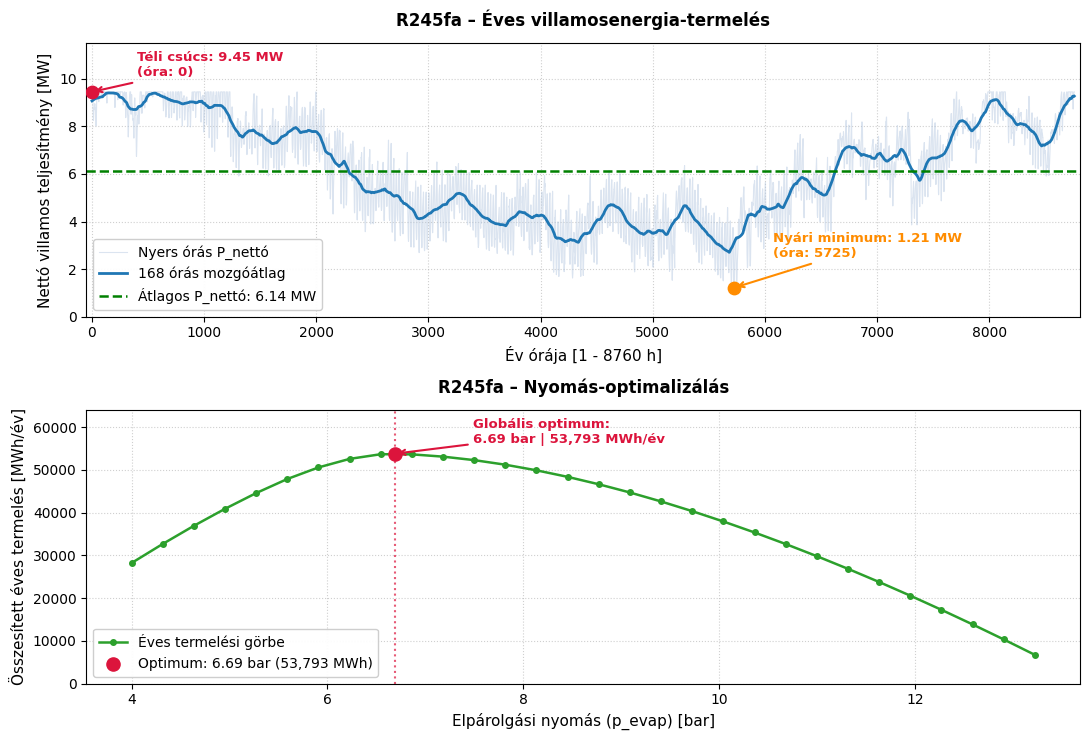
\includegraphics[width=0.85\textwidth]{R245fa.png}
    \caption{Az R245fa munkaközeg éves nettó villamosenergia-termelési dinamikája 168 órás mozgóátlaggal (fent), valamint az elpárolgási nyomás söprésének jelleggörbéje az optimális üzemállapot kijelölésével (lent).}
    \label{fig:R245fa}
\end{figure}

\begin{figure}[H]
    \centering
    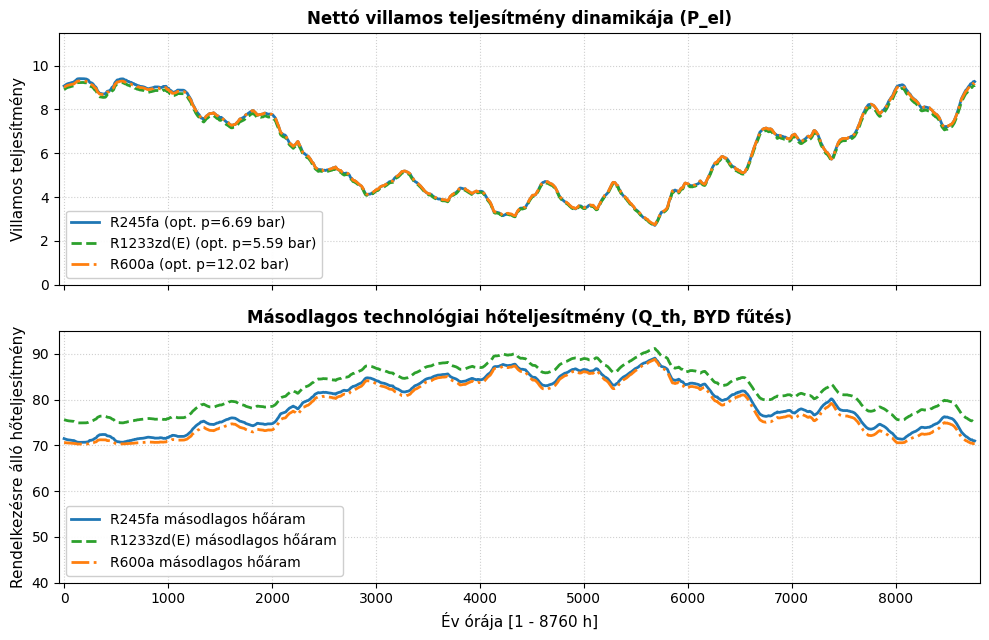
\includegraphics[width=0.85\textwidth]{hibrid.png}
    \caption{A kapcsolt hibrid üzemmód teljesítményprofiljai: az időjárásfüggő nettó villamos teljesítmény ($P_{\mathrm{el}}$) heti mozgóátlaga, valamint a másodlagos technológiai fűtésre kinyerhető stabil hőteljesítmény ($Q_{\mathrm{th}}$) az év 8760 órájában.}
    \label{fig:hibrid}
\end{figure}

\newpage \section{Gazdasági Értékelés és Környezeti Hatáselemzés}

\nocite{*}

\clearpage
\appendix
\section{Melléklet – Kiegészítő diagramok}

\begin{figure}[H]
    \centering
    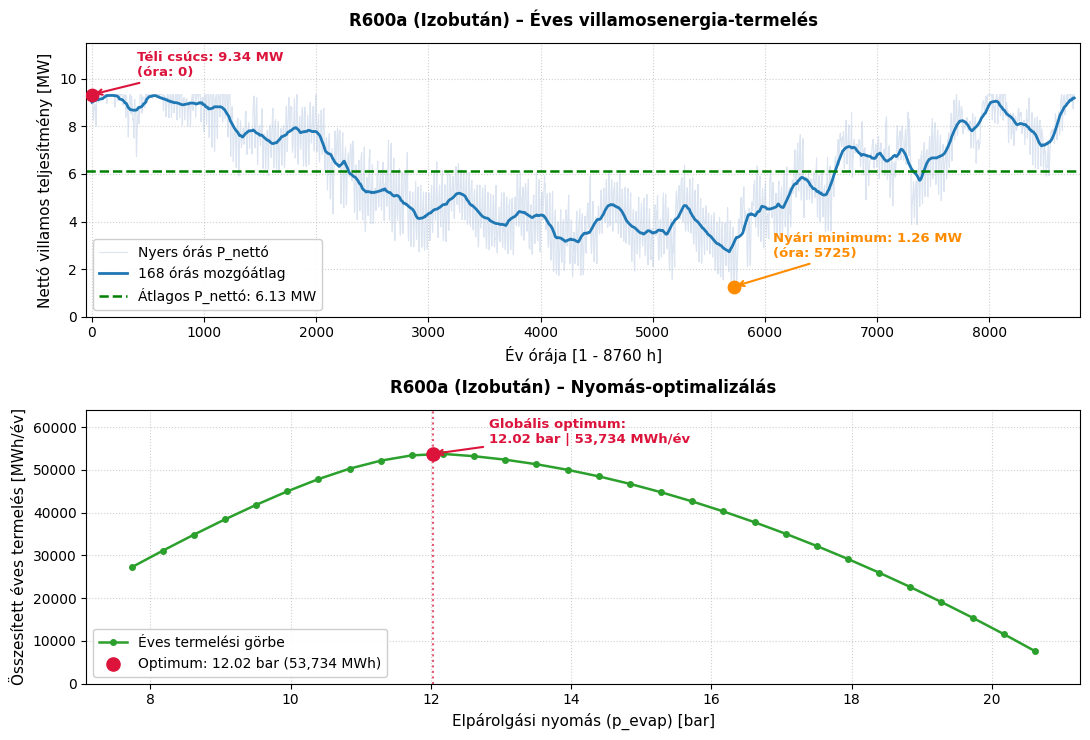
\includegraphics[width=0.85\textwidth]{R600a.png}
    \caption{Az R600a (izobután) munkaközeg éves nettó villamosenergia-termelési dinamikája 168 órás mozgóátlaggal (fent), valamint az elpárolgási nyomás söprésének jelleggörbéje az optimális üzemállapot kijelölésével (lent).}
    \label{fig:R600a}
\end{figure}

\begin{figure}[H]
    \centering
    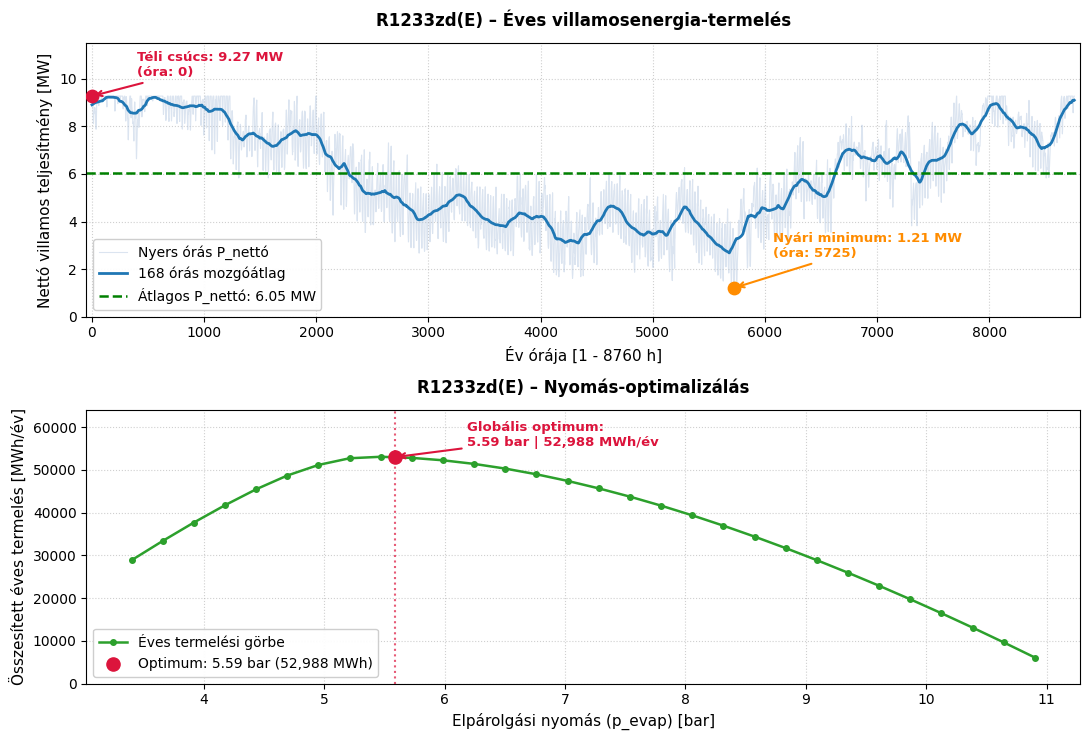
\includegraphics[width=0.85\textwidth]{R1233zdE.png}
    \caption{Az R1233zd(E) munkaközeg éves nettó villamosenergia-termelési dinamikája 168 órás mozgóátlaggal (fent), valamint az elpárolgási nyomás söprésének jelleggörbéje az optimális üzemállapot kijelölésével (lent).}
    \label{fig:R1233zdE}
\end{figure}

\end{document}